% !TeX root = ./algorithm_notes.tex
% chktex-file 46
% !TeX spellcheck = en-US
% !TeX encoding = utf8


\documentclass[]{article}

\RequirePackage{color,graphicx}
\usepackage{float}
\usepackage{longtable}
\usepackage{tabu}
\usepackage{pdfpages}
\usepackage{amsmath}
\usepackage{amsfonts}
\usepackage{amssymb}
\usepackage{mathtools}
\usepackage{csquotes}
\usepackage[american]{babel}
\usepackage[babel=true, protrusion=alltext-nott, final]{microtype}
\usepackage[nodayofweek]{datetime}
\usepackage[inline]{enumitem}
\usepackage{url}
\usepackage{todonotes}
\usepackage{biblatex}
\addbibresource{bibliography.bib}

%opening
\title{Corona Contact Tracing}
\author{Martin, Leonard, Thomas, Matthias}

\newcommand{\indexOfState}[1]{\texttt{indOfState}(#1)}
\DeclarePairedDelimiter\abs{\lvert}{\rvert}%
\DeclarePairedDelimiter\norm{\lVert}{\rVert}%

\setlength{\parskip}{1em}
\setlength{\parindent}{0cm}

\begin{document}

\maketitle

\begin{abstract}
	This technical report accompanies the implementation of the corona\_-contact\_tracing package found at \url{https://github.com/PellelNitram/corona_contact_tracing}.

	It extends an existing stochastic SIR simulation to generate data sets suitable to simulating the current corona pandemic.
	This simulation has full access to all agents' health status.
	To mirror a real world scenario the health status of agents is only partially observed through tests.

	Next we develop a graph convolutional approach to predict the health status of all agents in this simulation.
	It uses past contacts as well as oberved health information to derive this prediction.
	It is able to deal with partial data such as missing locations and missing health status, as it is a probabilistic approach.
	
	Lastly, this prediction can be used to derive measures to reduce the diseases' spread.
	We propose to find a optimal trade of between removing the least amount of edges in said graph (e.g. through quarantine, social distancing, etc.) and limiting the spread of the disease.
	% Such trade of could be found with minimal cut algorithms.
	Opposed to classical non-pharmaceutical intervention methods such as contact tracing, our approach directly identifies the nodes with the greatest potential to accelerate the diseases' spread in the network.
	
	This technical report was created within the \#WirVsVirus Hackathon of the German government and is Work in Progress!
\end{abstract}

\section{Algorithm notes}

\subsection{SIR Model}
Our basic stochastic SIR model relies on the assumptions that every person in an environment can be modeled as a point value, which has a location (i.e GPS coordinates) and an infection state. These states can be either \textit{susceptible} (S), \textit{infected} (I), \textit{recovered} (R) or in advanced models also \textit{under quarantine} (Q) or \textit{dead} (D). All individuals, here called agents, have a probability (here called diffusion rate $d$ to make a step per time step on a predefined grid. In the case, that some agents meet at the same location, disease spreading can occur. An infected agent spreads the disease with probability $\beta$ to all the agents in its close vicinity (same location on the grid). Furthermore recovery is covered by taking a recovery rate into account, i.e a probability $\gamma$ to recover from the disease per time step. If an infected agent recovers from the disease, the state of the agent changes from \textit{infected} to \textit{recovered}, which is definite (no double infections). The process ends, when no infected agents are left.
\begin{center}
    Susceptibles $\overset{\beta}{\longrightarrow}$ Infected $\overset{\gamma}{\longrightarrow}$ Recovered.
\end{center}

An example of a early model state is shown in Figure \ref{fig:1}
\begin{figure}[H]
    \centering
    \includegraphics[width=0.4\linewidth]{initial_setup.png}
    \caption{Early state of SIR model, blue dots = susceptibles, red dots = infected agents, green dots = Recovered agents}
    \label{fig:1}
\end{figure}

In this case, 1000 agents were initialized on a 100 by 100 grid, where a certain amount of infected agents were introduced as a seed. Letting the agents perform random walks on the grid (maximally one step each time step with probability $d$), and letting the model converge, the results in figure \ref{fig:2} can be observed.

\begin{figure}[H]
    \centering
    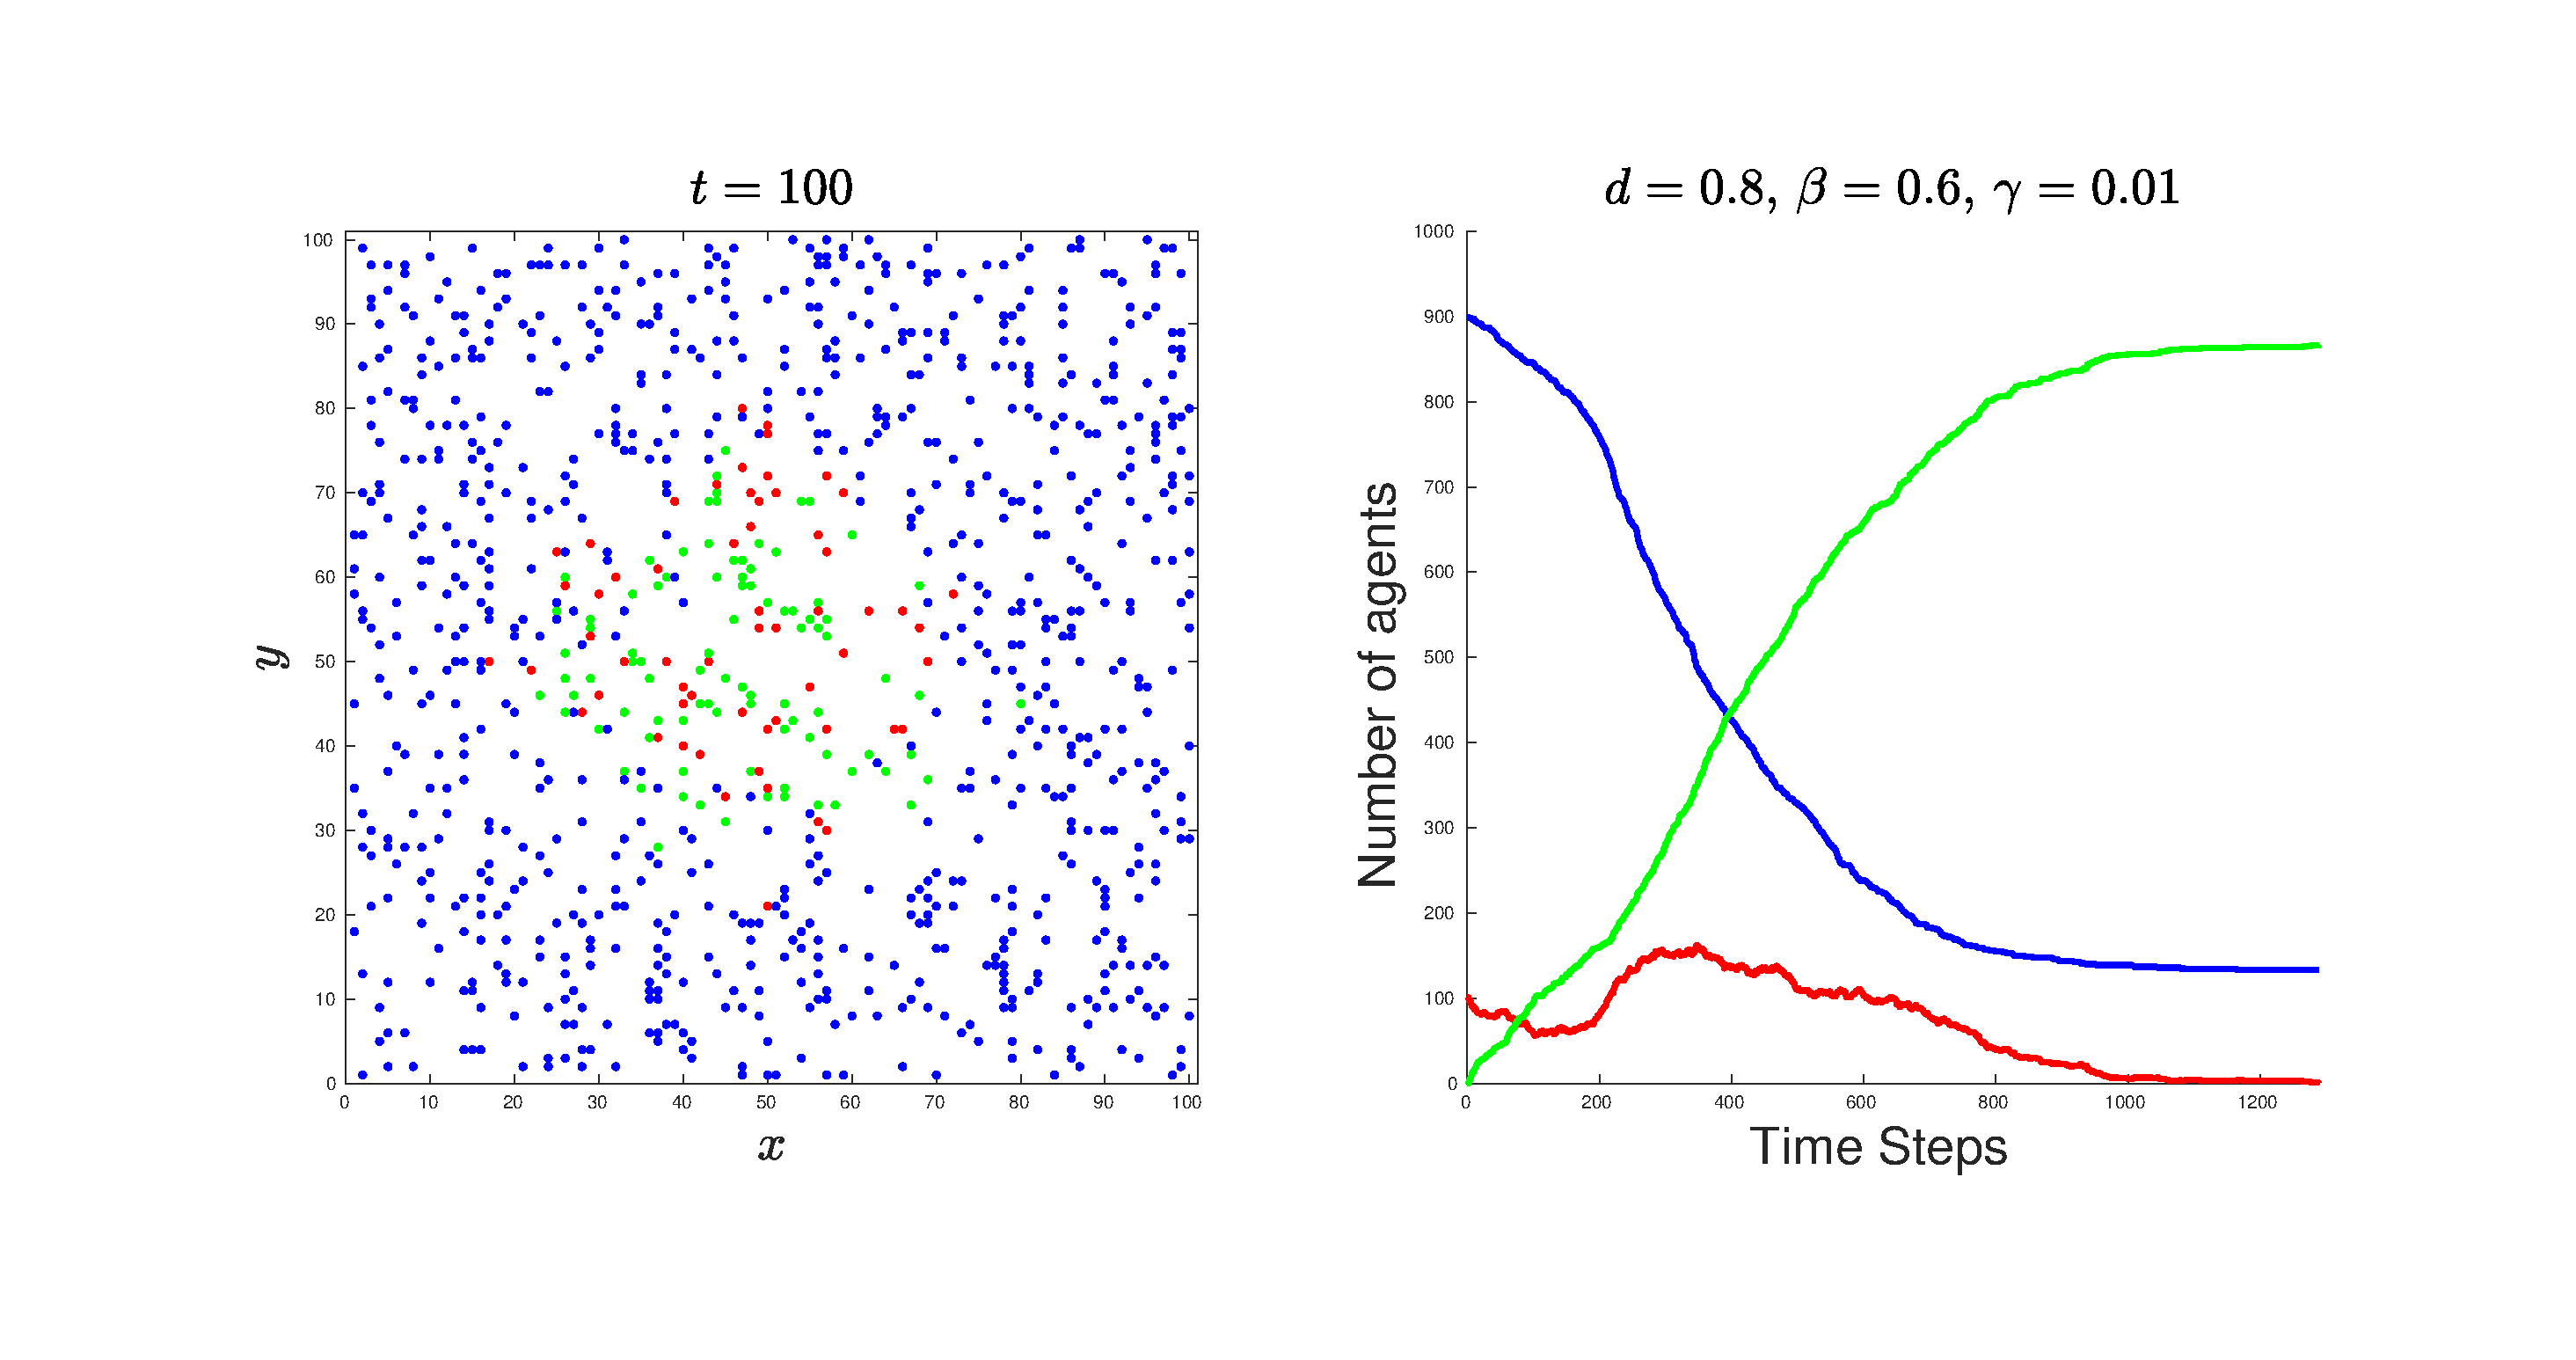
\includegraphics[width=0.9\linewidth]{1_1000_agents}
    \caption{Plot of the proportions of susceptible (blue), infected (red) and recovered (green) individuals in each state over time.}
    \label{fig:2}
\end{figure}

With the above stated parameters ($d=0.8$, $\beta=0.6$, $\gamma=0.01$), the disease does not spread over the whole population. However over 80\% were infected over time, which could be a very likely scenario of the corona out brake.


\subsection{Probabilistic Health Prediction}

We model partially infected populations as a graph, where each individual (interchangeably called agent) is a node. Edges of this graph model contacts of two agents. We use graph convolution, as explained below, to update our assumptions on the current health state of all individuals.

The definition of a graph convolution~\cite{Kipf2017SemiSupervisedCW} for here is

\begin{equation}
	\label{eq:graph_convolution}
	h_{v_i}^{(l+1)} = \sum_{j\in A(i)} h_{v_j}^{(l)}
\end{equation}

with feature vector $h$ of node $i$ from iteration $(l)$ to $(l+1)$. This formulation is equivalent to the matrix formulation $h^{(l+1)} = A h^{(l)}$ with $A$ as adjacency matrix as shown in section \ref{sec:consistency}. We consider here adjacency matrices without diagonal elements.

Our main propagation rule is based on the definition of a graph convolution shown in Eq.~\eqref{eq:graph_convolution} and reads as follows in component notation
\begin{equation}
	h_{v_i, m}^{(l+1)}
	=
	\underbrace{
		\sum_k \textcolor{red}{\frac{\hat{A}_{v_i, k}^{(l)}}{\sum_j \hat{A}_{v_i, j}^{(l)}}} h_{k, m}^{(l)} \textcolor{blue}{\delta_{m, e_I}}
	}_{\text{Graph}}
	+
	\underbrace{
		(h_{v_i}^{(l)}\cdot T)_m
	}_{\text{Temporal}}
\end{equation}

This propagation rule is based on the following aspects:

\begin{itemize}
	\item The propagation consists of two parts, first the graph contribution and second the temporal contribution. While the former captures the dynamics of infections based on the social contacts between agents, the former ensures that an infected agent heals over time and becomes resistant against the Corona virus.
	\item Each agent $i$ is modeled by $D$ features $h_{v_i}\in\mathbb{R}^D$. Therefore, the feature matrix, $h^{(l)}$, consists of all agents' features at time $(l)$ and is thereby of dimension $N\times D$ where there are $N$ agents in the population and each agent is described by $D$ features. A three dimensional feature space is used, $D=3$, modeling the three possible health states. The unit vectors of this space are interpreted as following:
	\begin{itemize}
		\item $\vec{e}_0$: susceptible state
		\item $\vec{e}_1$: infected state
		\item $\vec{e}_2$: recovered state
	\end{itemize}
	A uniform distribution over these possible states expresses complete uncertainty of the health state of an agent.
	\item Explanation of the graph contribution term:
	\begin{itemize}
		\item A sum over all agents' features $h_{k,m}^{(l)}$ is weighted by the normalised infection-adjusted graph connections as shown in red.
		\item The Kronecker delta, as shown in blue, ensures that only the I feature is added as this is the only one that matters during social contacts between agents.
		\item The infection-adjusted adjacency matrix $\hat{A}$ is constructed from $A$ and $I$ which are the regular continuous adjacency matrix and the infection matrix, respectively. These three quantities are explained in the following:
		\begin{itemize}
			\item The adjacency matrix $A$ is time dependent, $A^{(l)}$, and inferred from data. In our use case, $A_{ij} = \frac{1}{dist(v_i, v_j)+\epsilon}$, hence $A_{ij}$ is large when persons $i$ and $j$ have been in contact. $\epsilon$ serves as regularisation for small distances.
			\item The infection matrix is constructed as
			\begin{equation}
				I =
				\begin{pmatrix}
					0     &  0  & 0 \\
					\beta &  0  & \alpha \\
					0     &  0  & 0
				\end{pmatrix}
				=
				(I_{ij})_{i,j}
			\end{equation}
			with $i$ as the index of the host state and $j$ is the index of the contact person state. The states that we consider here are ordered as follows: susceptible, infected, recovered. $\beta$ denotes the probability of infection  after contact (also known as attack rate). $\alpha := 0$ models the probability of being reinfected, which we assume to be zero based upon current medical \todo{cite!}research.
			\item $\hat{A}$, with $\hat{A}_{ij}\in [0, 1]$, is the adjacency matrix that takes the infection interactions into account and is computed as follows
			\begin{equation}
				\hat{A}_{ij} = A_{ij}\cdot \frac{ h_{v_1}^T I h_{v_2} + h_{v_2}^T I h_{v_1} }{\beta}.
			\end{equation}
			The weighted scalar product of the health states of agents $i$ and $j$ is used to evaluate whether the edge is relevant for the infection dynamics. Only when an infected person and a susceptible have contact, the edge $A_{ij}$ should be considered, otherwise it should be dropped.	The sum in the denominator comes from the fact that both, agent $i$ and $j$, can act as host during a contact. The division by $\beta$ normalises the factor to one to ensure $\hat{A}_{ij} \in [0, 1]$. Since $I$ is not symmetric, $p_a$ is a proper normalisation because the sum is in $\{0, p_a\}$. Note that the fraction has the desired properties for pure $S$-, $I$- and $R$-persons.
		\end{itemize}
	\end{itemize}
	\item Explanation of the temporal term:
	\begin{itemize}
		\item The transition of a persons' health state $h_{v_i}^{(l)}$ is determined by the following assumptions:
		\begin{itemize}
			\item A susceptible person always stays susceptible
			\item An infected person has a probability $\gamma$, called recovery rate, to recover. The remaining probability $1-\gamma$ denotes that the person stays sick.
			\item A recovered person could have a probability to be re-infected, but we assume this to be zero. Thus a recovered person always stays recovered.
		\end{itemize}
		\item Thus the temporal transition matrix $T$ is:
		\begin{equation}
			T = 
			\begin{pmatrix}
				1 &     0    & 0      \\
				0 & 1-\gamma & \gamma \\
				0 &     0    & 1      \\
			\end{pmatrix}
		\end{equation}
		\item The temporal update rule based on the health status thus becomes:
		\begin{equation}
			H^{(l+1)} = H^{(l)} T
		\end{equation}
	\end{itemize}
\end{itemize}

\subsection{Disease Spread Reduction with Minimal Intervention}
This section presents approaches to optimally reduce the spread of the disease with minimal intervention.

\subsubsection{Edge Cutting Analysis}
All non pharmaceutical interventions (NPI) can be understood as some kind of edge removal in our graph-based approach:
\begin{itemize}
	\item Isolation of an infected individual removes all of its edges with very high probability.
	\item Quarantine of a contact person removes all of its edges with high probability.
	\item Social distancing removes some edges of of many individuals.
	\item Cancellation of large events remove many edges of many individuals.
\end{itemize}
As a first step analyze the effect of these measures in $R_0$.
$R_0$ models how many people are infected by a single infected person.
It is crucial to constrain $R_0$ below zero to avoid exponential growth in the number of infected individuals.


As future work we would like to explore ways to calculate the minimal set of edge removals which reduces the $R_0$ value of the pandemic below $1$.

In our approach $R_0$ can be derived from the ratio of infected people of $H^{(t+1)}$ and of $H^{(t)}$:
\begin{equation}
	R_0 = \frac{\norm{H^{(t+1)}\mid_{m=1}}_{0}}{\norm{H^{(t)}\mid_{m=1}}_{0}} %#TODO betrag
\end{equation}

The square matrix $C$ with dimensions $N \times N$ models desirable edge cancellations.
Note, that this matrix does not have to know the edges of a future time step, it only expresses which edges must not exist.
It is multiplied element-wise onto the adjacency matrix $A$, thus $\bar{A} = A \odot C$ describes a adjacency matrix with applied cancellations.

To optimally limit the spread of the disease, we seek to minimize the number of cancellations $\norm{C}_0$, given that $R_0$ is below zero:
\begin{equation}
	\max_{C} \norm{C}_0\text{, s.t. }R_0 < 1
\end{equation}

TODO: Derive an expanded statement from the above formulation.\\
% Future Work: This would be more powerful, if there would be some different kinds of edges (social, work, education, large events, etc.)\\
% Future Work: This only takes the current time step into account but it would be desirable to look even further into the future.

\subsubsection{Test Prioritization}
When tests are limited, they should be used to discover as much as possible about the health state of the overall population.
This in turn allows to reduce the $R_0$ value in further time steps as edge cutting is more efficient.

Lets assume there are $t_{\text{max}}$ tests per time step.
A test reveals the true health state of an individual (ignoring false negatives and false positives)
\begin{equation}
	h^{(t)} \xrightarrow{\text{test}} h^{(t+1)} \in \{\vec{e}_0, \vec{e}_1, \vec{e}_2 \}
\end{equation}

The test assignment $T$ with dimension $N$ is a binary variable describing which individuals should be tested.

\section{Appendix}

\subsection{Consistency of notations}
\label{sec:consistency}

Using the notation from the blog and the paper, including $H'\in\mathbb{R}^{N\times D}$, $A\in\mathbb{R}^{N\times N}$, $H\in\mathbb{R}^{N\times D}$, the propagation rule is:

\begin{equation}
	H' = A H
\end{equation}

is equivalent to

\begin{equation}
	\begin{split}
		H'_{v_i, m} & = \sum_l \overbrace{A_{v_i, l}}^{\in \{0, 1\}} H_{l, m} \\
		            & = \sum_{l'} H_{l',m}
	\end{split}
\end{equation}

where $l'$ takes all $A_{v_i,l}=1$, i.e. neighbours, into account.

Hence, I do understand that the notations are equal.

\subsection{Formulate normalisation}

Use from ICLR 2017 paper the normalisation $D_{ii} = \sum_j \hat{A}_{ij}$.

Use the knowledge from the blog post to write:

\begin{equation}
	\begin{split}
		\overbrace{H'}^{\in \mathbb{R}^{N\times D}} 
			& = \overbrace{D^{-1}}^{\in\mathbb{R}^{N\times N}} \overbrace{\hat{A}}^{\in \mathbb{R}^{N\times N}} \overbrace{H}^{\in\mathbb{R}^{N\times D}}
			\Leftrightarrow H'_{v_i, m} = \sum_k \overbrace{D^{-1}_{v_i,k}}^{=D_{v_i,v_i}, \delta_{v_i, k}} (\hat{A} H)_{km} \\
		& = D^{-1}_{v_i, v_i} (\hat{A} H)_{v_i, m} = D^{-1}_{v_i, v_i} \sum_k \hat{A}_{v_i, k} H_{k, m} = \sum_k \underbrace{\frac{\hat{A}_{v_i, k}}{\sum_j \hat{A}_{v_i, j}}}_{\text{normalised}} H_{k, m}.
	\end{split}
\end{equation}

The weighting by the adjacency matrix is, indeed, normalised to its column sums.

Note that this part is also normalised:

\begin{equation}
\begin{split}
	\sum_m H'_{v_i, m} & = \sum_m \sum_k \frac{\hat{A}_{v_i, k}}{\sum_j \hat{A}_{v_i, j}} H_{k, m} \\
	& = \sum_k \frac{\hat{A}_{v_i, k}}{\sum_j \hat{A}_{v_i, j}} \underbrace{\sum_m H_{k,m}}_{=1\text{, per construction}} = 1
\end{split}
\end{equation}

\printbibliography{}

\end{document}
